\documentclass[acmsmall]{acmart}
\usepackage{subcaption}
\usepackage{float}
\usepackage{tabularx}

%%
%% \BibTeX command to typeset BibTeX logo in the docs
\AtBeginDocument{%
  \providecommand\BibTeX{{%
    \normalfont B\kern-0.5em{\scshape i\kern-0.25em b}\kern-0.8em\TeX}}}

%% Rights management information.  This information is sent to you
%% when you complete the rights form.  These commands have SAMPLE
%% values in them; it is your responsibility as an author to replace
%% the commands and values with those provided to you when you
%% complete the rights form.
\setcopyright{none}
\copyrightyear{2020}
\acmYear{2020}
\renewcommand\footnotetextcopyrightpermission[1]{}
\acmDOI{}
\pagestyle{plain}
\settopmatter{printacmref=false}


%%
%% Submission ID.
%% Use this when submitting an article to a sponsored event. You'll
%% receive a unique submission ID from the organizers
%% of the event, and this ID should be used as the parameter to this command.
%%\acmSubmissionID{123-A56-BU3}

%%
%% The majority of ACM publications use numbered citations and
%% references.  The command \citestyle{authoryear} switches to the
%% "author year" style.
%%
%% If you are preparing content for an event
%% sponsored by ACM SIGGRAPH, you must use the "author year" style of
%% citations and references.
%% Uncommenting
%% the next command will enable that style.
%%\citestyle{acmauthoryear}

%%
%% end of the preamble, start of the body of the document source.
\begin{document}

%%
%% The "title" command has an optional parameter,
%% allowing the author to define a "short title" to be used in page headers.
\title{Author Attribution: DerStandard Forum Writing Style}

%%
%% The "author" command and its associated commands are used to define
%% the authors and their affiliations.
%% Of note is the shared affiliation of the first two authors, and the
%% "authornote" and "authornotemark" commands
%% used to denote shared contribution to the research.
\author{Patrick Deutschmann}
\email{patrick.deutschmann@tugraz.at}

\author{Lukas Timpl}
\email{lukas.timpl@tugraz.at}


%%
%% The abstract is a short summary of the work to be presented in the
%% article.
\begin{abstract}
  %TODO write abstract
\end{abstract}

%%
%% The code below is generated by the tool at http://dl.acm.org/ccs.cfm.
%% Please copy and paste the code instead of the example below.
%%
\begin{CCSXML}
<ccs2012>
   <concept>
       <concept_id>10010147.10010178.10010179</concept_id>
       <concept_desc>Computing methodologies~Natural language processing</concept_desc>
       <concept_significance>500</concept_significance>
       </concept>
 </ccs2012>
\end{CCSXML}

\ccsdesc[500]{Computing methodologies~Natural language processing}
%%
%% Keywords. The author(s) should pick words that accurately describe
%% the work being presented. Separate the keywords with commas.
\keywords{natural language processing, neural networks, author attribution, RNN}


%%
%% This command processes the author and affiliation and title
%% information and builds the first part of the formatted document.
\maketitle


\section{Author Attribution Problem Setting}

The aim of this project is to identify the authors of posts to a newspaper forum. This should be achieved through the incorporation of multiple factors, such as writing style and content, but also meta information such as the post date and the article to which the post was written. In that, the setting differentiates itself from the classical authorship attribution setting, where no meta information is used. 

The dataset we used for this project was the One Million Posts Corpus, provided by \cite{MillionPosts}. It contains user comments in German language posted for the Austrian newspaper DerStandard\footnote{\url{https://www.derstandard.at}}.

The concrete problem was formulated such that given a new post and its meta information, the most likely author of all forum users should be predicted. For that we only considered the most active users with at least 500 posts. There were in total 192 user for which this was the case in our data set.

\section{Related Work}

Authorship attribution is an actively researched field with many different special areas to focus on. While more traditional, manual methods such as described in \cite{criminalForensics} largely focus on linguistic expert analysis, more modern approaches make use of computers to solve the problem.

Much research effort, such as in \cite{rexha2015towards,sanderson2006short}, is focused on author attribution of far longer texts than the short ones given in our comments section. However, in \cite{smith2009authorship,macleod2012whose} there is some analysis of short texts with methods that are also applicable to our use case. 

This project differentiates itself from the aforementioned papers as it not only considers the writing style to determine the author, but also incorporates the meaning of the written text and some additional meta information, rendering it a significantly easier task.

\section{Setup}

This project explores different methods of identifying the authors of the forum posts. Due to the nature of the problem and the results obtained in previous work, we focused on investigating different structures of deep neural networks (multi-layer perceptrons). Other machine learning methods such as SVM or random forests are left for future work.

We implemented the neural network in Keras\footnote{\url{https://keras.io}} and used different architectures depending on which input features were considered. The contents of the posts used word embeddings and were then fed into a recurrent neural network, for which we obtained the best results using \textit{gated recurrent units} (GRU, proposed in \cite{gru}). They were later merged with the other features using a concatenation layer and propagated into a deep dense structure. The final predictions used a softmax activation to determine the most likely author. To prevent overfitting, we used dropout layers as a means of regularisation.

For training, we used Adam \cite{adam} as the optimiser and categorical cross-entropy loss, as we posed our problem as a multi-class classification. The network structures and features are explained in detail in the following section. 

\section{Features}
To best utilise our dataset, we made use of various different features which are described in this section. 

\subsection{Post Metadata}
The dataset contains a number of values we consider as metadata, data that is not directly related to the actual text of the post and can be computed without considering the actual content of the post. 

\subsubsection{Date Statistics}
For this feature we analysed at which time of the day and on which day of the week users write their posts. 
The notion behind this was that individual users will tend to post at similar times.
A histogram of this data is depicted in Figure~\ref{fig:date_stats}.

\begin{figure}
\centering
\begin{subfigure}{.5\textwidth}
\centering
  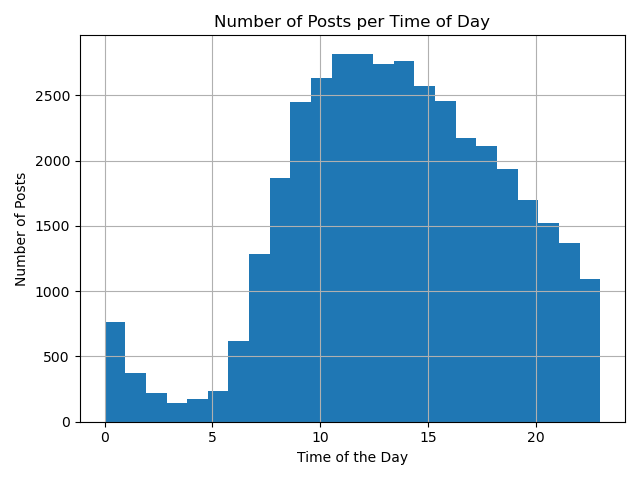
\includegraphics[width=.9\linewidth]{assets/Number_of_posts_per_time_of_day.png}
 \end{subfigure}%
\begin{subfigure}{.5\textwidth}
\centering
  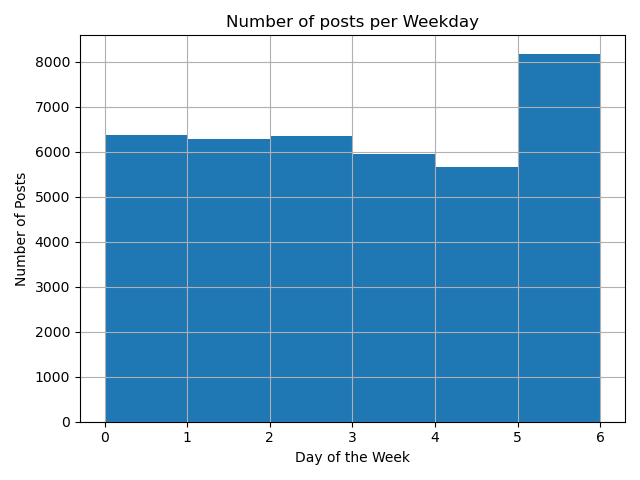
\includegraphics[width=.9\linewidth]{assets/Number_of_posts_per_day_of_week.png}
 \end{subfigure}
 \caption{Date Statistics}
\label{fig:date_stats}
\end{figure}

\subsubsection{Post Ratings and Parent Posts}
For further information about a post without the actual content we looked at the post ratings and whether the post was a comment to another user's post. The aim with this feature was to identify users that post more controversial content as well as users that only ever post comments (have a parent post) and users that never answer to other users (no parent post). Again we depict a histogram over this data (Figure~\ref{fig:post_stats}). This figure clearly shows that most posts get no votes at all, while there are a few posts which get a very large number of votes. 

\begin{figure}
\centering
\begin{subfigure}{.5\textwidth}
\centering
  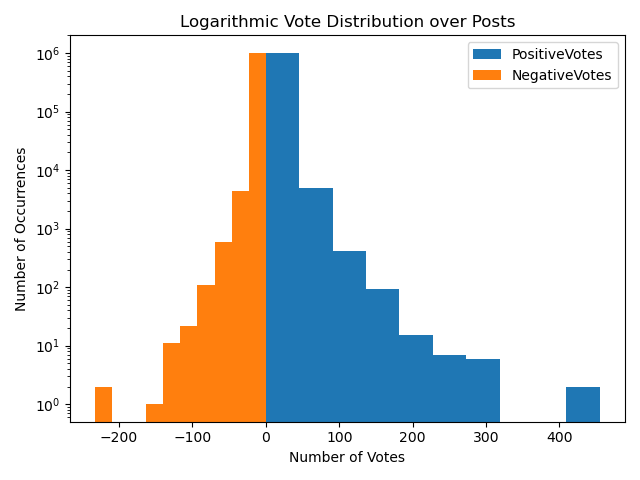
\includegraphics[width=.9\linewidth]{assets/Logarithmic_Vote_Distribution_over_Posts.png}
 \end{subfigure}%
\begin{subfigure}{.5\textwidth}
\centering
  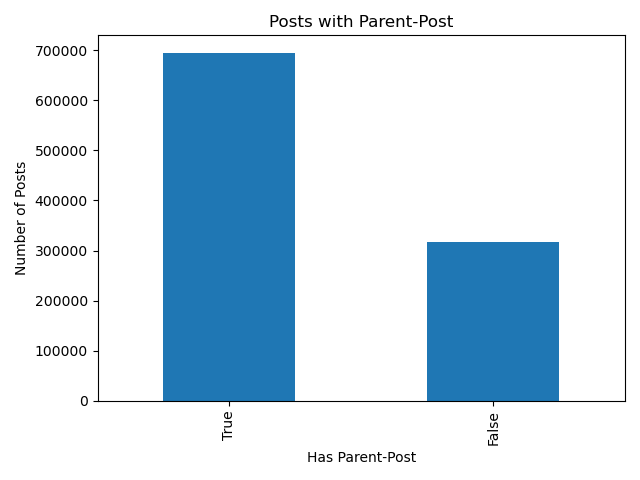
\includegraphics[width=.9\linewidth]{assets/Posts_with_parent_post.png}
 \end{subfigure}
 \caption{Post Statistics}
\label{fig:post_stats}
\end{figure}

\subsubsection{Article Categories}
For every given post, our data set contains the article it belongs to. Articles in the dataset also contain a path which we used as a categorical feature with the idea that individual users will be more interested in particular topics and therefore are more likely to write post under those articles. A histogram of the number of articles in each category of the most common main category "Newsroom" is depicted in Figure~\ref{fig:article_categories}.

\begin{figure}[H]
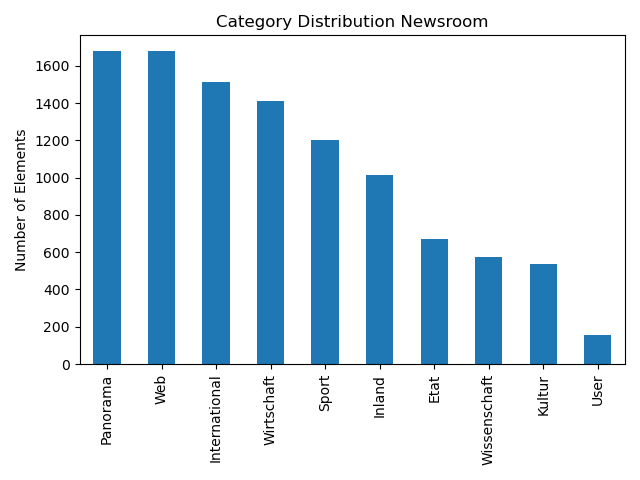
\includegraphics[width=.5\linewidth]{assets/Category_Distribution_Newsroom.png}
\caption{Article Category Distribution}
\label{fig:article_categories}
\end{figure}


\subsubsection{Article Named Entities}
To get a more detailed view of the interests of users additionally to the article categories, we also analysed named entities in the articles under which the posts were written. Similarly to the article categories, the notion behind this was that individual users will be more interested in certain entities and hence are more likely to write a post under articles containing these Entities. \\
For this, we utilised the library Flair\footnote{\url{https://github.com/flairNLP/flair}}, a library that offers state-of-the-art Named Entity Recognition for the German language. Histograms for the most frequently recognised entities are depicted in Figure~\ref{fig:named_entities}. We only used entities that occurred at least 20 times. We count the occurrences of each entity and encode each article as a vector containing all entity counts. 

\begin{figure*}[h!]
        \centering
        \begin{subfigure}[b]{0.475\textwidth}
            \centering
            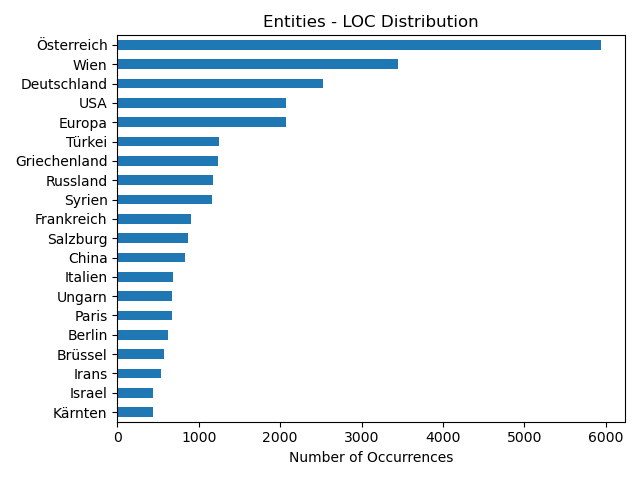
\includegraphics[width=\textwidth]{assets/Entities_LOC_Distribution.png}
        \end{subfigure}
        \begin{subfigure}[b]{0.475\textwidth}  
            \centering 
            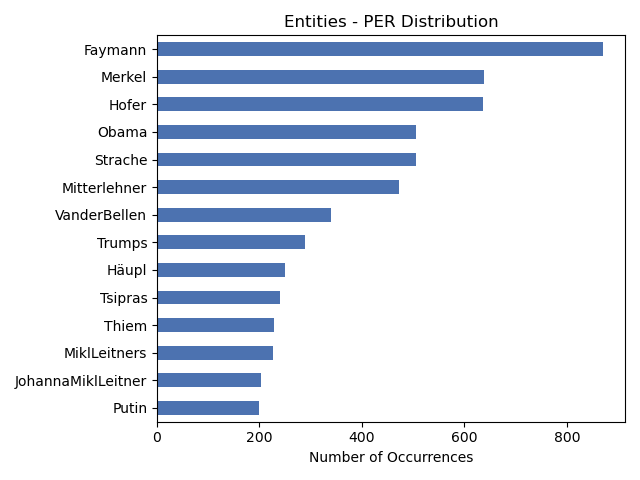
\includegraphics[width=\textwidth]{assets/Entities_PER_Distribution.png}
        \end{subfigure}
        \begin{subfigure}[b]{0.475\textwidth}   
            \centering 
            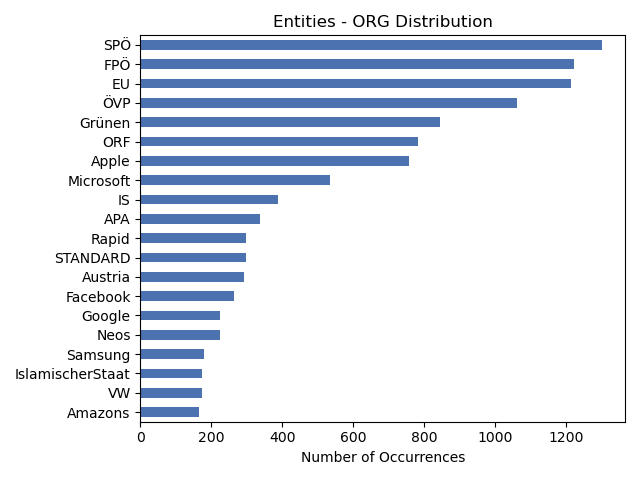
\includegraphics[width=\textwidth]{assets/Entities_ORG_Distribution.png}
        \end{subfigure}
        \begin{subfigure}[b]{0.475\textwidth}   
            \centering 
            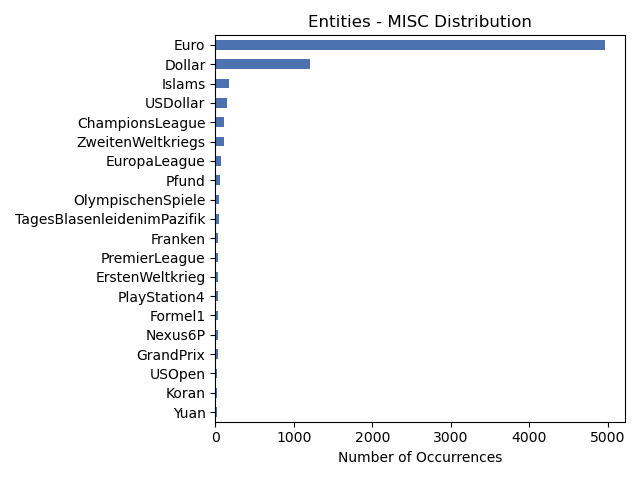
\includegraphics[width=\textwidth]{assets/Entities_MISC_Distribution.png}
        \end{subfigure}
         \caption{Top Entities in Articles for locations (LOC), persons (PER), organizations (ORG) and other Entities (MISC).}
         \label{fig:named_entities}
\end{figure*}


\subsection{Stylometric}
Next, we looked at the content of the posts and computed various stylometric features. These features are based on the writing style of the user. The list and description of these features can be found in Table~\ref{tab:stylometric}. We computed all of those features twice. Once for the headline of the post and once for the actual text. The notion behind this is, that we noticed that the way in which the headline was used differed significantly between users. While some users choose to leave the field empty, some showed a clear tendency towards upper-case characters, and some wrote the headline as the start for the main text and concluded it with "...". 

\begin{table}[H]
\begin{tabularx}{\textwidth}{lX}
Feature Name & Description \\ \hline
Alpha-chars-ratio & The fraction of total characters in the paragraph which are letters \\
Digit-chars-ratio & The fraction of total characters in the paragraph which are digits \\
Upper-chars-ratio & The fraction of total characters in the paragraph which are upper-case \\
White-chars-ratio & The fraction of total characters in the paragraph which are whitespaces \\
Emoticon-chars-ratio & The number of Emoticons (e.g. ":)", ":D", ...) per total characters \\
Average-word-length & Average length of words in characters \\
Average-sentencechar-length & Average length of sentences in characters \\
Average-sentenceword-length & Average length of sentences in words \\
Total length & The length of the text \\
\end{tabularx}
\caption{Used Stylometric Features}
\label{tab:stylometric}
\end{table}

\subsection{Post Embeddings}
As a final feature, we computed word embeddings for the post texts. The goal of this feature is to get information on the actual content the users write about as well as potentially additional information on their writing style. \\
To compute the vectors, we utilized the Word2Vec model of the library Gensim\footnote{\url{https://radimrehurek.com/gensim/}}. 
We used embedding vectors of size 50, only computed the embeddings for words which at least occurred ten times and trained the model over 500 iterations. 
When embedding the posts, we only embedded at most 100 words for each post to restrict the size of the feature.  

\section{Evaluation}
In this section we describe our results. For the final training of the network, we split into a test and training set (80\%/20\%). Additionally we used a validation dataset for early stopping (20\%) of the training test. 

\subsection{Baseline}
%TODO find more baseline data
The most apparent lower bound baseline is random guessing. In our dataset we have 192 Users, hence a random guess yields an accuracy of $1/192 = 0.0052$. 

\subsection{Results}
In this section, we list the achieved results for various feature configurations. For all our trained models, we tried different architectures in terms of the number of neurons and the number of layers. Furthermore, we tested different hyperparameters, such as learning rate and drop-out regularization. We used early stopping to determine the ideal amount of training epochs. If the validation accuracy did not improve for three consecutive epochs, we stopped the training and restored the weights to the ones that achieved the highest accuracy. \\
We first trained models for each individual feature to find out how much it contributed to the classification accuracy. The chosen hyper parameters as well as the corresponding results are listed in Table~\ref{tab:result_features}. 
Next we trained different configurations containing various combinations of features. These results with the chosen hyper parameters are depicted in Table~\ref{tab:result_configurations}.

\subsubsection{Individual Features}
To get an idea of the usefulness of individual features we trained the network for each individual feature. 

For all features below, we trained a simple network using an input layer, one or two hidden layers and one output layer. 
The results for each feature and the corresponding parameters are listed in Table~\ref{tab:result_features}.

\begin{table}[H]
\begin{tabular}{lllllll}
Feature & Val. Acc. & Test Acc. & Layers & Dropout & Learning Rate & Epochs\\ \hline
Date Stats & 0.041 & 0.047 & (256) & - & 0.2 & 20 \\
Post Ratings & 0.042 & 0.044 & (512) & - & 0.2 & 4 \\
Parent Post & 0.041 & 0.039 & (256) & - & 0.2 & 7 \\
Article Categories & 0.090 & 0.087 & (190) & - & 0.1 & 8 \\
Article Entities & 0.26 & 0.26 &  (700)  & - & 0.2 & 6 \\
Stylometric & 0.21 & 0.21 & (150),(512) & - & 0.1 & 18 
\end{tabular}
\caption{Results for individual features}
\label{tab:result_features}
\end{table}

We found that the named entities in the article and the stylometric features of the post itself achieved the highest accuracies on their own.

\subsubsection{Metadata Features}
The notion behind this model was to use all available features that are not related to the content of the post. Therefore, the following features are used:
\begin{itemize}
\item Date Statistics
\item Post Ratings
\item Parent Posts
\item Article Categories
\item Article Named Entities
\end{itemize}
Even without the actual content of the post, just using the user response and the entities of the corresponding article, this model was able to achieve a decent test accuracy of $0.27$. 

\subsubsection{Dense Features}
This model contains all features except for the post embeddings. Since we added recurrent layers for the post embeddings, this is the configuration with all features such that the model is still a feed-forward network. We call the configuration \textit{Dense Features} as its inputs are only sent through dense layers. \\
By adding the stylometric features when compared to the model before, this configuration was also able to incorporate information about the writing style of users, which allowed it to perform even better achieving a test accuracy of $0.35$.


\subsubsection{Post Content Features}
Since this model utilised the post embeddings, we added recurrent layers and a concatenation layer to merge them with the remaining features which are only used in a feed-forward manner. 
The model is depicted in Figure~\ref{fig:post_content_model}.
This model contains all features which are directly related to the content of the post.
Therefore the following features are used:
\begin{itemize}
\item Post Embeddings
\item Stylometrics
\end{itemize}
This configuration only utilized the actual user posts, however with the addition of the post embeddings and a more complex architecture it was able to identify users significantly better than a model which just used stylometrics (see Table~\ref{tab:result_features}). It achieved a test accuracy of $0.31$.


\subsubsection{All Features}
For this model, we combined all available features. We used a recurrent network for the post embeddings and combined it with a feed-forward network of the other features. The model is depicted in Figure~\ref{fig:complete_model}. This model was able to significantly outperform all other configurations and achieved a test accuracy of $0.44$.


\begin{table}[H]
\begin{tabular}{lllllll}
Configuration & Val. Acc. & Test Acc. & Layers & Dropout & Learning Rate & Epochs\\ \hline
Metadata Features & 0.28 & 0.27 & (512) &  - & 0.2 & 18 \\
Dense Features & 0.36 & 0.35 & (90),(512) & - & 0.2 & 12 \\
Post Content Features & 0.32 & 0.31 & Fig.~\ref{fig:post_content_model} & 0.3 & 0.2 & 8 \\
All Features & 0.45 & 0.44 & Fig.~\ref{fig:complete_model} & 0.3 & 0.2 & 11 \\
\end{tabular}
\caption{Results for Configurations}
\label{tab:result_configurations}
\end{table}

\begin{figure}[H]
\centering
\begin{subfigure}{.5\textwidth}
\centering
  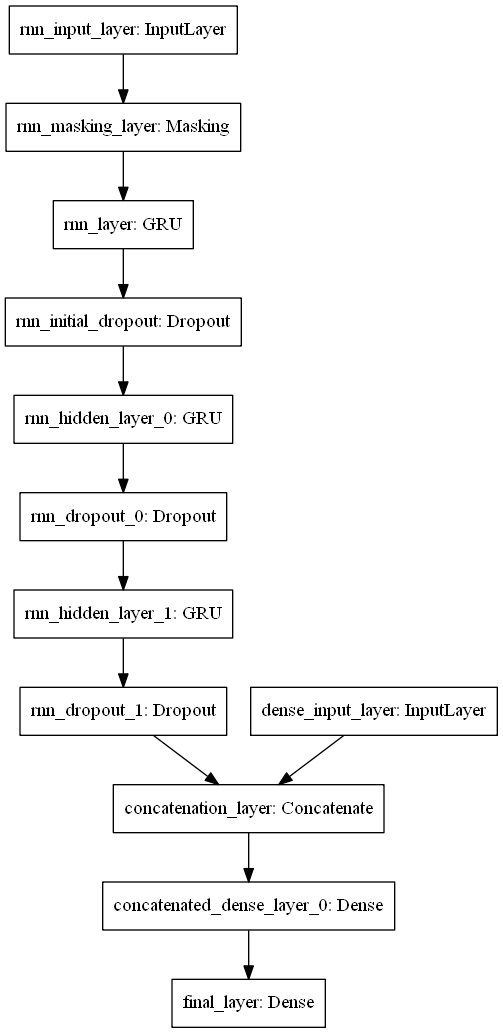
\includegraphics[width=.9\linewidth]{assets/AuthorAttributionModel_post_content_features.png} 
  \caption{Model for Post Content Features}
  \label{fig:post_content_model}
 \end{subfigure}%
\begin{subfigure}{.5\textwidth}
\centering
  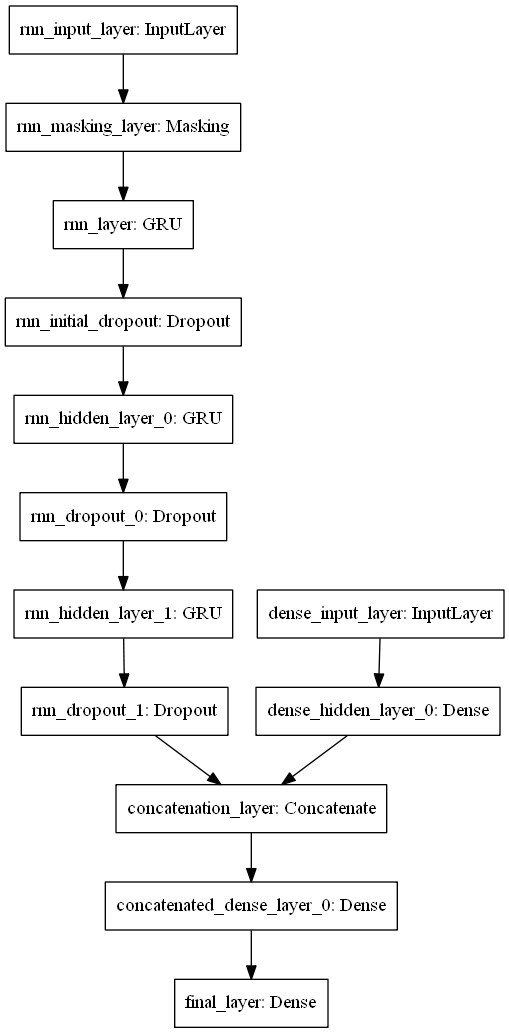
\includegraphics[width=.9\linewidth]{assets/AuthorAttributionModel_all_features.png}
  \caption{Complete Model for all features}
    \label{fig:complete_model}
 \end{subfigure}
 \caption{RNN Models}
\label{fig:rnn_models}
\end{figure}


\section{Discussion}

In this section, we discuss the successes and challenges of our results and possible explanations.

\subsection{Feature selection}

In terms of feature selection, the statistics on post dates were less helpful than we had expected. We conclude that users either don't have a clear enough posting routine to make accurate predictions or that there wasn't enough information for the number of users between we were distinguishing. However, they performed still around seven times better than random guessing. 

The contents of the posts (i.e. the word embeddings of the posts and the named entities in the corresponding articles) haven proven to yield very good results. In comparison, however, they also required the highest pre-processing efforts. The article entities in particular have shown to be well suited for capturing users' interests. That this is very helpful for predicting comment authorship was also shown by the article categories, which, despite being rather simple features, delivered a performance around 17 times better than random guessing. It was also quite helpful that the named entities in the articles captured quite well what the articles were about, as embedding the whole articles would have significantly enlarged the input vectors and hence made the network harder to train.

Stylometric features also worked quite well for our prediction, even though we only used very simple ones. Most likely, better results could be obtained for more advanced features, such as vocabulary richness measures. We leave these to future work.

\subsection{Data preparation}

This task very heavily relied on data preparation for successful predictions. For the article categories, it was essential to one-hot-encode them before feeding them into the network. Also, we performed some normalisation on the date statistics as, for example, just putting in the raw timestamp of the posts created severe perturbations in the training.

As already alluded to above, the post embeddings required significant pre-processing. We found prior stemming useful to detect entities, as, for example, "Amazons" refers to the same entity as "Amazon", but is used in a different case. To prevent feature vectors from growing too large, we found it important to only consider to the most common entities. 

\subsection{Network architecture and hyper parameters}
Our final results used a multi-input neural network with two input branches, one feed-forward and one recurrent for the post embeddings. We found it important to include another dense layer after the concatenation of both branches to allow the network to learn the balance between the features.

The recurrent network took significantly longer to train and our available hardware resources put limits to the extent of our hyper-parameter search. While we already explored many options, future work might explore different choices and hence yield better results. We found GRU units to outperform LSTM, which proved to be harder to train. 

While dropout worked well as a means of regularisation in the recurrent branch of the network, for the feed-forward part, we found it more useful to keep the network simple by restricting the number of layers and neurons in order to keep the model from overfitting. We further mitigated issues of overfitting by using early stopping.

\section{Conclusion}

Overall, we conclude that we obtained rather good results for the given task. However, as this project is an application, it was hard to find a perfectly apt baseline to compare to. An important part of the good results is attributed to incorporating the semantics of the posts and articles into the prediction task. We found a wide variety of different features combined to yield the best results for our setting. 

%TODO

% TODO write about future work:
% - try architectures other than Neural Network (MLP)
% - comparison with other methods

\section{Appendix}


\subsection{User Response Prediction}

\subsubsection{Problem Setting}
This problem aims to predict the response to user posts based on the article content. Effectively we want to predict the number of positive and negative votes that user posts under an article will receive. 

\subsubsection{Setup}
We implemented our network using Keras. We decided to use a simple feed-forward network. We experimented with different architectures both in terms of the number of layers as well as the number of neurons per layer. To prevent overfitting, we used early stopping where we stopped the training if the loss function value on the validation set did not decrease for two consecutive epochs. 

\subsubsection{Features}
As features, we used the Named Entities of the articles. We only selected entities which occurred at least five times and also restricted the articles to ones containing at least five entities. 

\subsubsection{Targets}
The distribution of our targets is depicted in Figure~\ref{fig:user_resp_targets}. The votes are distributed extremely uneven and are best captured on a logarithmic scale. This also leads to our decision to use the mean squared logarithmic error (logarithmic MSE) as a loss function. Otherwise, our network would completely neglect articles which receive fewer votes. Additionally, we monitored the mean absolute error (MAE) to get an easier understandable however also less fair error metric.  

\begin{figure}[H]
\centering
\begin{subfigure}{.5\textwidth}
\centering
  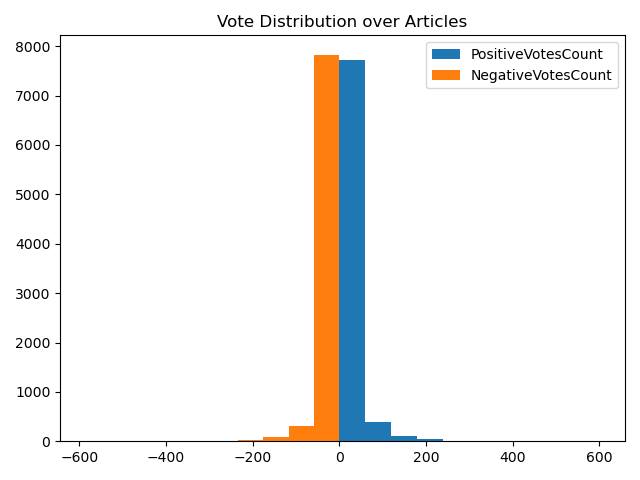
\includegraphics[width=.9\linewidth]{assets/Vote_Distribution_over_Articles.png} 
  \caption{Vote distribution over articles}
  \label{fig:vote_distribution_articles}
 \end{subfigure}%
\begin{subfigure}{.5\textwidth}
\centering
  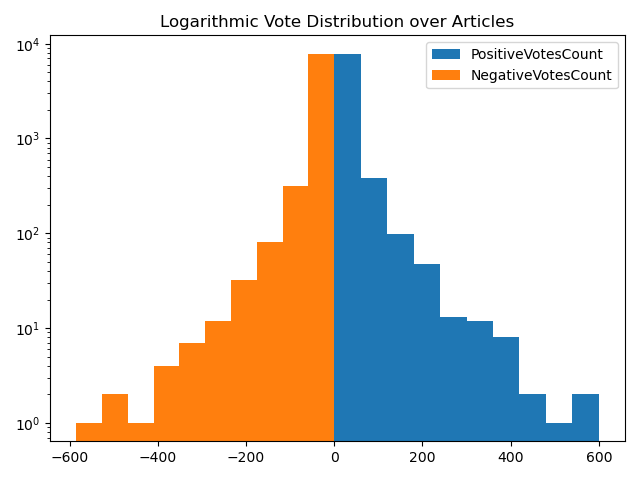
\includegraphics[width=.9\linewidth]{assets/Logarithmic_Vote_Distribution_over_Articles.png}
  \caption{Logarithmic vote distribution over articles}
    \label{fig:log_vote_distribution_articles}
 \end{subfigure}
 \caption{Targets for user response prediction}
\label{fig:user_resp_targets}
\end{figure}

\subsubsection{Evaluation}
We split our data into a training and test set (80\%/20\%) and used a part of the training data (20\%) as a validation set. After some experiments, we decided on a simple architecture consisting of one input layer, one output layer and two hidden layers, both with four neurons. We used a small batch size of 10 and the Adam optimizer. Since the network performed very fast during training, we found that we can use a relatively very small learning rate of $1 \times 10^{-5}$, which gave use slightly better results than larger ones. \\
The training results are depicted in Figure~\ref{fig:training_results}. In the beginning, we see a steady decline both in the loss values and also in the validation loss. However, with an increasing amount of iterations, the validation loss no longer decreases, and the network starts to overfit, at which point the early stopping stops the training. 
The final result on the test set is a logarithmic MSE of $1.9$ and an MAE of $13.8$.

\begin{figure}[H]
\centering
\begin{subfigure}{.5\textwidth}
\centering
  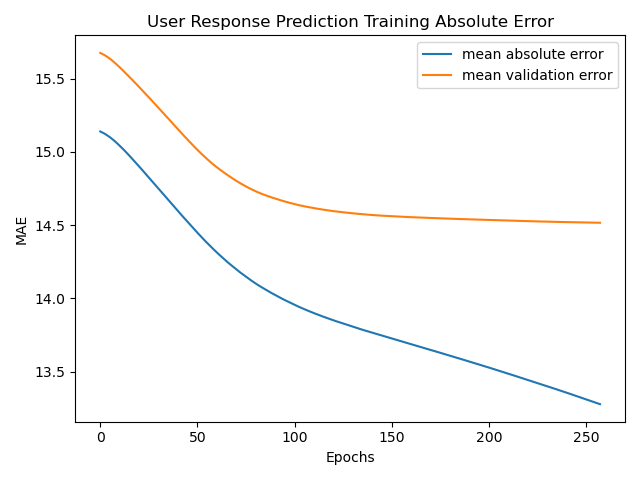
\includegraphics[width=.9\linewidth]{assets/User_Response_Prediction_Training_Absolute_Error.png} 
  \caption{Absolute absolute error over training iterations}
 \end{subfigure}%
\begin{subfigure}{.5\textwidth}
\centering
  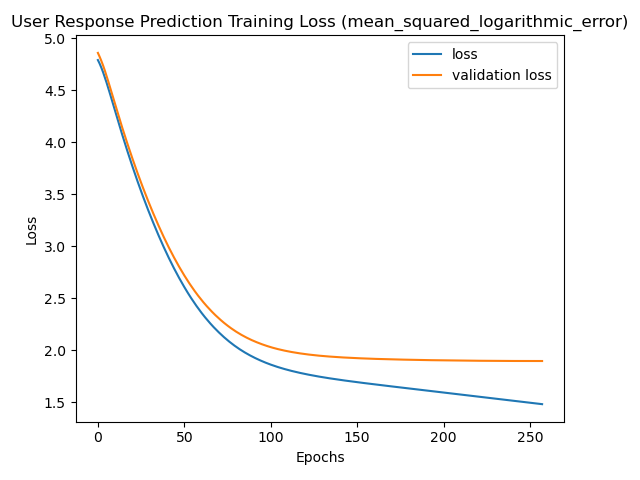
\includegraphics[width=.9\linewidth]{assets/User_Response_Prediction_Training_Loss_mean_squared_logarithmic_error_.png}
  \caption{Logarithmic MSE over training iterations}
 \end{subfigure}
 \caption{Training results}
\label{fig:training_results}
\end{figure}

\subsection{Named Entity Analysis}
Additionally, to using Named Entities as features for our networks, we also performed some other experiments. For example, we analysed the occurrences of entities in articles over time (Figure~\ref{fig:per_entities_over_time}). \\ Furthermore, we calculated a co-occurrence matrix for the occurrences of entities in articles. From this matrix, we constructed a graph using the tool Gephi~\footnote{\url{https://gephi.org}}, which allowed us to analyse connections between entities. A part of this graph with entities connected to Österreich is depicted in Figure~\ref{fig:graph_cooccurrences_oesterreich}.

\begin{figure}[H]
\centering
\begin{subfigure}{.5\textwidth}
\centering
  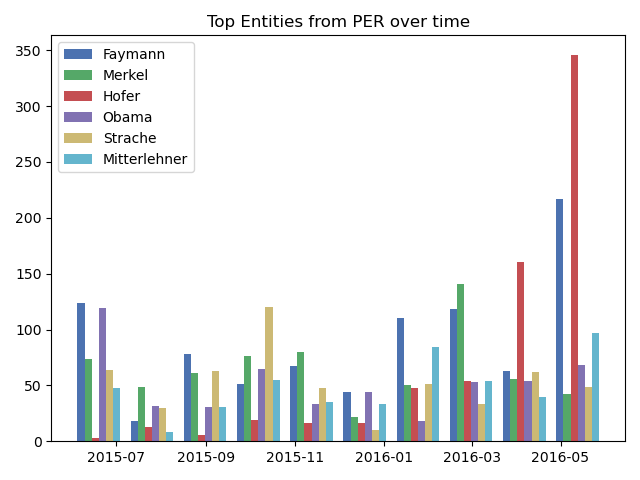
\includegraphics[width=.9\linewidth]{assets/Top_Entities_from_PER_over_time.png} 
  \caption{Frequency of top entities with label person over time}
  \label{fig:per_entities_over_time}
 \end{subfigure}%
\begin{subfigure}{.5\textwidth}
\centering
  \includegraphics[width=.9\linewidth]{assets/co_occurrences_österreich.png}
  \caption{Entities connected to Österreich in Gephi}
  \label{fig:graph_cooccurrences_oesterreich}
 \end{subfigure}
 \caption{Named Entity analysis}
\label{fig:ne_analysis}
\end{figure}



\pagebreak

%%
%% The next two lines define the bibliography style to be used, and
%% the bibliography file.
\bibliographystyle{ACM-Reference-Format}
\bibliography{references}


\end{document}
\endinput

